\section{Using \padx{} to Query Ad Hoc Data}
\label{section:padx}

\begin{figure}
\begin{center}
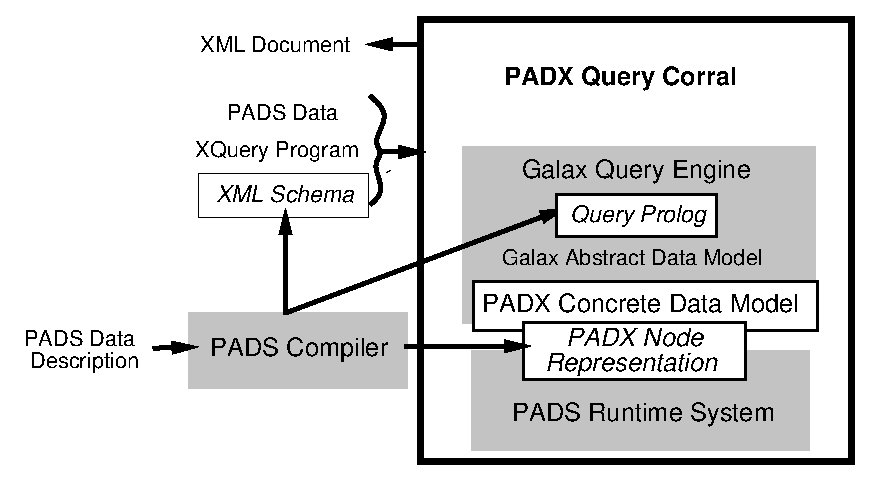
\epsfig{file=padx-arch.ps,width=0.47\textwidth}
\end{center}
\caption{Internal view of \padx{} Architecture}
\label{figure:padx-arch}
\end{figure}

Figure~\ref{figure:padx-arch} depicts an internal view of the \padx{}
architecture first shown in Figure~\ref{figure:padx-arch1}.
Pre-existing components (in grey boxes) include the \pads{} compiler,
the \Galax{} query engine, and the \pads{} runtime system.  In this
section, we focus on the new components (in white boxes) and describe
the compiler and run-time support for viewing \pads{} data as XML.
From a \pads{} description, the compiler generates an XML Schema
description that specifies the virtual XML view of the corresponding
\pads{} data; an XQuery prolog that imports the generated schema and
that associates the input data with the correct schema type; and a
type-specific library that provides the virtual XML view of \pads{}
values necessary to implement \padx{}'s concrete data model.  

Note that a query corral is \emph{customized} for a particular \pads{}
description, in particular, its concrete data model only supports
views of data sources that match the \pads{} description.  To maintain
the correct correspondence between a description, XML Schema, queries,
and data, the query corral explicitly contains the generated query
prolog, which imports the XML Schema that corresponds to the
underlying type-specific library.  This guarantees that the user's
XQuery program is statically typed, compiled, and optimized with
respect to the correct XML Schema and that the underlying data model
is an instance of this XML Schema.  At runtime, the query corral takes
an XQuery program and a \pads{} data source and produces the query
result in XML.  We discuss the problem of producing native \pads{}
values in Section~\ref{section:future}.

\subsection{Viewing \pads{} data as XML}	

The mapping from a \pads{} description to an XML Schema is 
straight-forward.  The interesting aspect of this mapping is that both
\pads{} values that are error free and those containing errors are
accessible in the XML view.  We begin with the mapping of \pads{} base
types. 

A default XML Schema, \cd{pads.xsd}, contains the schema types that
represent the \pads{} base types shared by all \pads{} descriptions.
Figure~\ref{figure:pads.xsd} contains a fragment of this schema.
Every \pads{} base type is mapped to the schema simple type that most
closely subsumes the value space of the given \pads{} base type.  For example,
the \cd{Puint32} base type maps to the schema type \cd{xs:unsignedInt}
(Lines~1--3).  Recall that all parsed \pads{} values have an in-memory
representation and a parse descriptor, which records the state of the
parse, the error code for detected errors, and the location of those
errors.  The XML view of a parsed value is a choice of the in-memory
representation (\cd{rep}), if no error occurred, or of the parse
descriptor (\cd{pd}), if
an error occurred (Lines~4--8).  This light-weight view exposes the
parse descriptor only when an error occurs.  The parse-descriptor type
for all base types is represented by the schema type
\cd{Pbase\_pd} (Line~10--14).

\begin{figure}
\begin{small}
\begin{code}
 1. <xs:simpleType name="\kw{base\_Puint32}">
 2.  <xs:restriction base="\kw{xs:unsignedInt}"/>
 3. </xs:simpleType>
 4. <xs:complexType name="\kw{val_Puint32}">
 5.  <xs:\kw{choice}>
 6.   <xs:element name="\kw{rep}" type="\kw{p:base\_Puint32}"/>
 7.   <xs:element name="\kw{pd}"  type="\kw{p:Pbase_pd}"/>
 8.  </xs:\kw{choice}>
 9. </xs:complexType>
{10}. <xs:complexType name="\kw{Pbase_pd}">
{11}.  <xs:sequence>
{12}.   <xs:element name="\kw{pstate}"  type="\kw{p:Pflags_t}"/>
{13}.   <xs:element name="\kw{errCode}" type="\kw{p:PerrCode_t}"/>
{14}.   <xs:element name="\kw{loc}"     type="\kw{p:Ploc_t}"/>
{15}.  </xs:sequence>
{16}. </xs:complexType>
\end{code}
\end{small}
\caption{Fragment of XML Schema for \pads{} base types.}
\label{figure:pads.xsd}
\end{figure}

The fragment of the XML Schema in Figure~\ref{figure:dibbler-schema}
corresponds to the description in Figure~\ref{figure:dibbler}.  Note
that the schema imports the schema for \pads{} base types (Line~5).
Each compound type is mapped to a complex schema type with a
particular content model.  A \kw{Pstruct} is mapped to a complex type
that contains a sequence of local elements, each of which corresponds
to one field in the \kw{Pstruct}.  For example, the \kw{Pstruct}
\cd{order\_header\_t} is mapped to the complex type
\cd{order\_header\_t} (Lines~7--15), which contains an element
declaration for the field \cd{order\_num}, among others.  A
\kw{Punion} is mapped to a complex type that contains a choice of
elements, each of which corresponds to one field in the \kw{Punion}.
\begin{figure*}
\begin{small}
\begin{code}
{ 1}. <xs:schema targetNamespace="\kw{file:/example/sirius.p}"
{ 2}.            xmlns="file:/example/sirius.p"
{ 3}.            xmlns:xs="http://www.w3.org/2001/XMLSchema"
{ 4}.            xmlns:p="http://www.padsproj.org/pads.xsd">
{ 5}. <xs:import namespace = "\kw{http://www.padsproj.org/pads.xsd}".../>
{ 6}. ...
{ 7}. <xs:complexType name="\kw{order_header_t}">
{ 8}.  <xs:sequence>
{ 9}.   <xs:element name="\kw{order_num}"     type="\kw{p:val_Puint32}"/>
{10}.   <xs:element name="\kw{att_order_num}" type="\kw{p:val_Puint32}"/>
{11}.   <xs:element name="\kw{ord_version}"   type="\kw{p:val_Puint32}"/>
{12}.   <!-- More local element declarations -->
{13}.   <xs:element name="\kw{pd}"            type="\kw{p:PStruct_pd}" minOccurs="0"/>
{14}.  </xs:sequence>
{15}. </xs:complexType>
{16}. <!-- More complex type declarations -->
{17}. <xs:complexType name="\kw{orders_t}">
{18}.  <xs:sequence>
{19}.   <xs:element name="\kw{elt}"    type="\kw{order_t}" maxOccurs="unbounded"/>
{20}.   <xs:element name="\kw{length}" type="\kw{p:Puint32}"/>
{21}.   <xs:element name="\kw{pd}"     type="\kw{p:Parray_pd}" minOccurs="0"/>
{22}.  </xs:sequence>
{23}. </xs:complexType>
     ...
{24}. <xs:element name="\kw{Psource}" type="\kw{summary_t}"/>
{25}. </xs:schema>
\end{code}
\end{small}
\caption{Fragment of XML Schema for \dibbler{} \pads{} description.}
\label{figure:dibbler-schema}
\end{figure*}

Each complex type also includes an optional \cd{pd} element that
corresponds to the type's parse descriptor (Lines~13 and~21).  All
parse-descriptor types contain the parse state, error code, and
location.  The parse-descriptor for compound types contain additional
information, \eg{}, \cd{Pstruct\_pd} contains the number of nested
errors and \cd{Parray\_pd} contains the index of the array item in
which the first error occurred.  The \cd{pd} element is absent if no
errors occurred during parsing, but if present, permits an analyst to
easily identify the kind and location of errors in the source data.
For example, the following XQuery expression returns the locations of all
orders that contain at least one error:
\cd{$pads/Psource/orders/elt/pd/loc}.

The schema types for some compound types contain additional fields
from the \pads{} in-memory representation, \eg{} arrays have a length
(Line~20).  Note that \cd{Parray} types do not associate a name with
each individual array item, so in the corresponding schema type, the
default element \cd{elt} encapsulates each array item.

The \pads{} compiler generates a query prolog that specifies the
environment in which all XQuery programs are typed and evaluated. 
Figure~\ref{figure:padx-query-prolog} contains the query prolog for
the schema in Figure~\ref{figure:dibbler-schema}.  The import schema
declaration on Line~1 imports the schema in
Figure~\ref{figure:dibbler-schema}.  This declaration puts all global
element and type declarations in scope for the query.  The variable
declaration on Line~2 specifies that the value of the variable
\cd{\$pads} is provided externally and that its type is a document
whose top-level element is of type \cd{Psource}, defined on Line~24 in
Figure~\ref{figure:dibbler-schema}.  This declaration guarantees
that the query is statically typed with respect to the correct input type.

At run time, the user can specify
the input data as a command-line argument or by calling the XQuery
\cd{fn:doc} function on a \pads{} source, \eg{} \cd{pads:/example/sirius.data}.
\begin{figure*}
\begin{small}
\begin{code}
 1. import schema default element namespace "\kw{file:/example/sirius.p}";
 2. declare variable \kw{$pads} as \kw{document-node(Psource)} external; 
\end{code}
\end{small}
\caption{\padx{} generated query prolog}
\label{figure:padx-query-prolog}
\end{figure*}

\subsection{\padx{} Concrete Data Model}

In Figure~\ref{figure:padx-arch}, the interface between \Galax{} and
\pads{} consists of two modules: the generic \padx{} concrete data model,
which implements the \Galax{} abstract data model, and a
compiler-generated module, in which each \pads{} type has a
corresponding, type-specific node representation providing the XML
view of values of that type.

Figure~\ref{fig:padx-element-node} contains a fragment of the \padx{}
concrete data model for a node.  This object provides a thin wrapper
around the type-specific node representation, \cd{padx\_node\_rep},
whose interface is in Figure~\ref{fig:padx-node-rep}.  A node
representation contains references to a \pads{} value's in-memory
representation and parse descriptor.  The node representation
interface returns the \Xml{} view of the \pads{} value, including the
value's element name, its typed value, and parent.
The \cd{kth\_child} and \cd{kth\_child\_by\_name} methods 
return all of the \pads{} value's children in order and those with a
given name in order, respectively.
\begin{figure*}
\begin{small}
\begin{code}
class virtual \kw{padx\_node\_rep} :
  object 
    (* Private data includes parsed value's rep \& pd *)
    method node\_name   : unit -> string
    method typed\_value : unit -> item
    method parent       : unit -> padx\_node\_rep option
    method \kw{kth\_child}   : int -> padx\_node\_rep option
    method \kw{kth\_child\_by\_name} : int -> string -> padx\_node\_rep option
  end
\end{code}
\end{small}
\caption{The \padx{} node representation}
\label{fig:padx-node-rep}
\end{figure*}

For some methods in Figure~\ref{fig:padx-element-node} (Lines~4--5),
the concrete data model simply invokes the corresponding type-specific
methods.  One exception is the \cd{child} axis method (Lines~7--17),
which we describe in detail as it illustrates how the \Xml{} view of a
\pads{} source is materialized lazily.
The \cd{child} method takes an optional name-test argument.  We
describe the case when the name-test is absent, which corresponds to
the common expression \cd{child::*}.  The \cd{child} method creates a
mutable counter \cd{k} (Line~8), which contains the index of the
last child accessed, and a function \cd{lazy\_child} (Lines~11--16),
which is invoked each time the \cd{child} cursor is poked.  On each
invocation, \cd{lazy\_child} increments the counter and delegates to
the \cd{kth\_child} method of the type-specific node representation.
For some \pads{} types, accessing the virtual \nth{k} child does not
require reading or parsing data, \eg{} if the virtual child is part of
a complete \pads{} record.  For other \pads{} types, \eg{} \kw{Parray}s that
contain file records, accessing the virtual \nth{k} child may require
reading and parsing data.  The \cd{kth\_child} method provides a
uniform interface to all types and delegates the problem of when to
read and parse data to the underlying type-specific node
representation.
\begin{figure*}
\begin{small}
\begin{code}
{ 1}. class \kw{pads\_node} (\kw{nr} : \kw{padx\_node\_rep}) =  
{ 2}. object 
{ 3}.   inherit Galax.node
{ 4}.   method node\_name   () = nr#node\_name()
{ 5}.   method typed\_value () = nr#typed_value() 
{ 6}.   (* ... Other data model accessors ... *)
{ 7}.   method \kw{child} name\_test =  
{ 8}.     let \kw{k} = ref 0 in
{ 9}.     match name\_test with 
{10}.     | None ->  
{11}.       let \kw{lazy\_child} () = 
{12}.        (incr k;
{13}.         match \kw{nr#kth\_child} \kw{!k} with
{14}.         | Some cnr ->  Some(new pads\_node(cnr))
{15}.         | None -> None)
{16}.       in Cursor.cursor\_of\_function lazy\_child
{17}.     | Some (NameTest name) -> 
            (* Same as above, but call nr#kth\_child\_named *)
{18}.   (* ... Other axes ... *)
{19}. end
\end{code}
\end{small}
\caption{Fragment of the \padx{} concrete data model}
\label{fig:padx-element-node}
\end{figure*}

To illustrate type-specific compilation, we give the
compiler-generated node representation of an \cd{order\_header\_t}
value in Figure~\ref{fig:order-node-rep}.  The object takes the name
of the field that contains the \cd{order\_header\_t} value, which
corresponds to the \Xml{} node name, and the in-memory representation
and parse descriptor of the value.  The \cd{kth\_child} method
(Lines~9--15) takes an index and returns the node representation of
the field at that index.  For example, the first child (Line~11)
corresponds to the field \cd{order\_num}, which contains a
\kw{Puint32} value.  The \cd{kth\_child\_by\_name} method
(Lines~16--21) provides constant-time lookup of a child with a
particular name: It looks up the index of the name in the associative
map \cd{name\_map} and then delegates to \cd{kth\_child}.  Note that
this \Xml{} view of an \cd{order\_header\_t} value corresponds to the
schema type \cd{order\_header\_t} in
Figure~\ref{figure:dibbler-schema}.

\cut{This example is representative of \kw{Pstruct}s.  
The node representations of \kw{Punions} and \kw{Parray} types.}

To summarize, the \padx{} \condm{} completely implements the \Galax{}
data model, making it possible to evaluate any XQuery program over a
\pads{} data source.  Due to limited space, we have omitted some
details, such as how \padx{} guarantees that each virtual node has a
unique, immutable identity, as is required by the \Galax{} \absdm{}.
The data model's most important features are that it provides lazy
access to virtual \Xml{} nodes in the \pads{} source, it delegates
navigation to type-specific node representations, and it separates
navigation of the virtual nodes from data loading, which is discussed
next.

\begin{figure*}
\begin{small}
\begin{code}
{ 1}. class \kw{order\_header\_t\_node\_rep}
{ 2}.       (field\_name : string)
{ 3}.       (rep : order\_header\_t)
{ 4}.       (pd  : order\_header\_t\_pd) = 
{ 5}. object 
{ 6}.   inherit padx\_node\_rep
{ 7}.   method name() = field\_name
{ 8}.   ... 
{ 9}.   method \kw{kth\_child} idx = 
{10}.     match idx with 
{11}.     |  1 -> Some(new val\_Puint32\_node\_rep("order\_num", rep.order\_num, pd.order\_num\_pd))
{12}.     |  2 -> Some(new val\_Puint32\_node\_rep("att\_order\_num", rep.att\_order\_num, pd.att\_order\_num\_pd))
{13}.     | ...
{14}.     | 14 -> Some(new Pstruct\_pd\_node\_rep("pd", pd))
{15}.     | _  -> None
\mbox{}
{16}.   (* Chidren's name map *)
{17}.   let \kw{name_map} = Associative\_array.create [("order\_num", 1); ("att\_order\_num", 2); ...; ("pd", 14)] 
{18}.   method \kw{kth\_child\_by\_name} child\_name =
{19}.     match Associative\_array.lookup name\_map child\_name with
{20}.     | None -> Cursor.empty_cursor()
{21}.     | Some idx -> kth_child idx 
{22}. end
\end{code}
\end{small}
\caption{Fragment of compiler-generated node representation for \texttt{order\_header\_t}}
\label{fig:order-node-rep}
\end{figure*}

\subsection{Loading \pads{} data}
% Connect scalability to the "multiple entry point parsing routines" in
% Sec 2:
% \begin{itemize}
% \item galax has a "virtual random-access view" of the XML
%   source. Interface to PADX does not reveal details of how and when
%   data is loaded. The interface puts no restrictions on access.
% \item Indeed, \padx{} can supply a real random-access view of the data but at a
%   high cost. Can prefetch entire data source into memory, but then
%   depend on VM system to manage any overflows. Call this prefetch {\em
%     bulk load}.
% \item Problems crop up early due to quantity of data generated (on
%   average) per byte.
% \item Therefore, bulk reading will only work for the smallest of
%   data sets.
% \item This drawback is not a flaw in the system, but an intentionally
%   chosen point in the design space. The parsing libraries were never
%   intended to be used that way. Instead, \pads model is for programmer
%   to use multiple entry points to control the parsing to produce
%   manageable quantities of data. \pads generates a lot of meta data
%   and lets programmer filter as desired.
% \item Unfortunately, requires much programmer involvement. We want to
%   capitilize on this behaviour, but automatically, without requiring
%   any more involvement by Galax than what is already provided in
%   interface. so we use the libraries as intended by reading
%   sequentially and maintaining just enough state to satisfy
%   Galax. That is, we take advantage of multiple entry points provided,
%   but in an automatic way.
% \item In fact, the automatic nature of the \padx memory management,
%   offers a value-added tool to even the ``pure'' \pads
%   programmer. However, the memory management layer is not free, as we
%   now examine in more detail.
% \end{itemize}

The \padx{} \absdm{} provides \Galax{} with a random-access view of a
\pads{} data source. In particular, any virtual node may be accessed
in any order at any time during query evaluation regardless of its
physical location in the \pads{} data.  This abstraction permits the
\padx{} \condm{} to decide when and how to read and parse, or \emph{load},
a data source.  \cut{The only requirement is that the \padx{} \condm{}
guarantee that each virtual node has a unique, immutable identity,
as is required by the \Galax{} \absdm{}.}

\padx{} has three strategies for loading data, each of which use the
multiple-entry parsing functions generated by the \pads{} compiler.
The \emph{bulk} strategy loads a complete \pads{} source before query
evaluation begins, populating all the in-memory representations and
parse descriptors.  With all data pre-fetched, bulk loading is the
simplest strategy to implement genuine random access.  However,
because each \pads{} value has quite a bit of associated meta-data, bulk
loading incurs a high memory cost and is only feasible for smaller
data sources.

The \emph{on-demand, random-access} strategy loads \pads{} data when
\Galax{} accesses virtual nodes via the \absdm{}.  The strategy
maintains a fixed size buffer for loaded values and when the buffer is
filled, expels values in LIFO order.  The default units for loading
are any \pads{} types annotated with \kw{Precord}, which indicates
that the type denotes an atomic physical unit in the ambient coding.
This default works well in practice, because many \pads{} sources
contain a header, one (or more) very large array(s) of records, and a
trailer.  This strategy loads all the data before the record array(s)
and then loads each array item on demand, expelling old records when
the buffer is filled.  A small amount of meta-data is preserved for
each expelled record, so that the virtual node containing that data
can be reconstructed on subsequent accesses.

The \emph{on-demand, sequential} strategy is a restriction of the
on-demand, random-access strategy.  It loads data on demand, but its
fixed-size buffer stores only one record at a time, and it supports
strictly sequential access to records, \ie{} accessing records out of
order is prohibited.  Given that the \Galax{} \absdm{} requires random
access, it is not obvious when this strategy can be used, even though
it has the smallest memory footprint of all three and, therefore,
could scale to very large sources.  It turns out that many common
XQuery queries can be evaluated in \emph{one} sequential scan over the
input document, and in these cases, the sequential strategy is
semantically correct and also time and space efficient.  We give
examples of ``one-scan'' queries and their performance in the next
section.

\cut{It too maintains
a fixed amount of storage space (one record) and loads on demand. However, it
supports strictly sequential access -- neither skipping ahead, nor
rewinding is allowed.  Many common queries permit sequential,
  streamed access to underlying XML source.  Give an example.}

\cut{This rep permits multiple
scans of input, but slowly. Does not work for read once data that can't be
``rewound'' such as live streams.

In sum, the following three data loading schemes are supported by \padx:

\begin{enumerate}
\item Bulk loading: Materialize entire \pads{} representation, populate all
  of the \pads reps. Build \padx \condm upon memory-resident data.

\item On-demand sequential loading: Keep storage for one record. Read
  records on demand into single memory slot. Strictly sequential.

\item On-demand, random access loading: Store fixed number of records in
  memory at any one time. Allow access to arbitrary records in
  arbitrary order.
\end{enumerate}}

\cut{
support the random-acccess view with true random access to the data by
prefetching the entire data source into memory, before any calls to
the \padx \absdm are made. 
Indeed, bulk loading is the simplest approach to data materialization.
Unfortunately, it can also be quite costly.  As long as the entire
data source along with its \pads meta-data fit comfortably in memory,
prefetching is cost-effective. However, once the memory requirements
push on the virtual memory system, performance plummets.

The question, then, is how often do we have to worry about data
sources hogging memory. The answer, unforunately, is quite often.
Problems crop up early due to quantity of data that \pads generates
(on average) per byte. Therefore, bulk loading is only practical for
the smallest of data sets.

This restriction, however, should not be seen as a flaw in \pads, but
an intentionally chosen point in the design space. The generated
parsing libraries were never intended to be used for bulk loading
large data sources. Instead, the \pads model is for the programmer to
use the multiple entry points of the generated parsing library to
parse manageable quantities of data at at time. \pads generates a lot
of meta data and lets the programmer filter it as desired.

Unfortunately, this model requires a great deal of programmer
involvement. We need a way to load data according to the \pads model,
but automatically, without requiring any more involvement by Galax
than what is already provided in interface. To accomplish this, we
build a layer of data loading ``intelligence'' between \galax and the
\padx parsing library.  This layer uses the library as intended by
keeping a fixed amount of data in memory at any point, and loading
new data upon request from \galax.

However, for performance reasons, we provide two implementations of
the loading-management layer. The first is semantically true to the
bulk loading mechanism, supporting random access to the data. {\em
  details}.System preserves meta-data about previously read records,
but re-uses memory for reading next item.  This rep permits multiple
scans of input, but slowly. Does not work for read once data that can't be
``rewound'' such as live streams.

The second approach is an optimization of the first. It too maintains
a fixed amount of storage space (one record) and loads on demand. However, it
supports strictly sequential access -- neither skipping ahead, nor
rewinding is allowed. {\em should note here that this last option is
  not fully implemented. macros exist, but compiler doesn't spit out
  function definitions.}   Many common queries permit sequential,
  streamed access to underlying XML source.  Give an example.

In sum, the following three data loading schemes are supported by \padx:

\begin{enumerate}
\item Bulk loading: Materialize entire \pads{} representation, populate all
  of the \pads reps. Build \padx \condm upon memory-resident data.

\item On-demand sequential loading: Keep storage for one record. Read
  records on demand into single memory slot. Strictly sequential.

\item On-demand, random access loading: Store fixed number of records in
  memory at any one time. Allow access to arbitrary records in
  arbitrary order.
\end{enumerate}
}